\begin{figure}[H]
\centering
  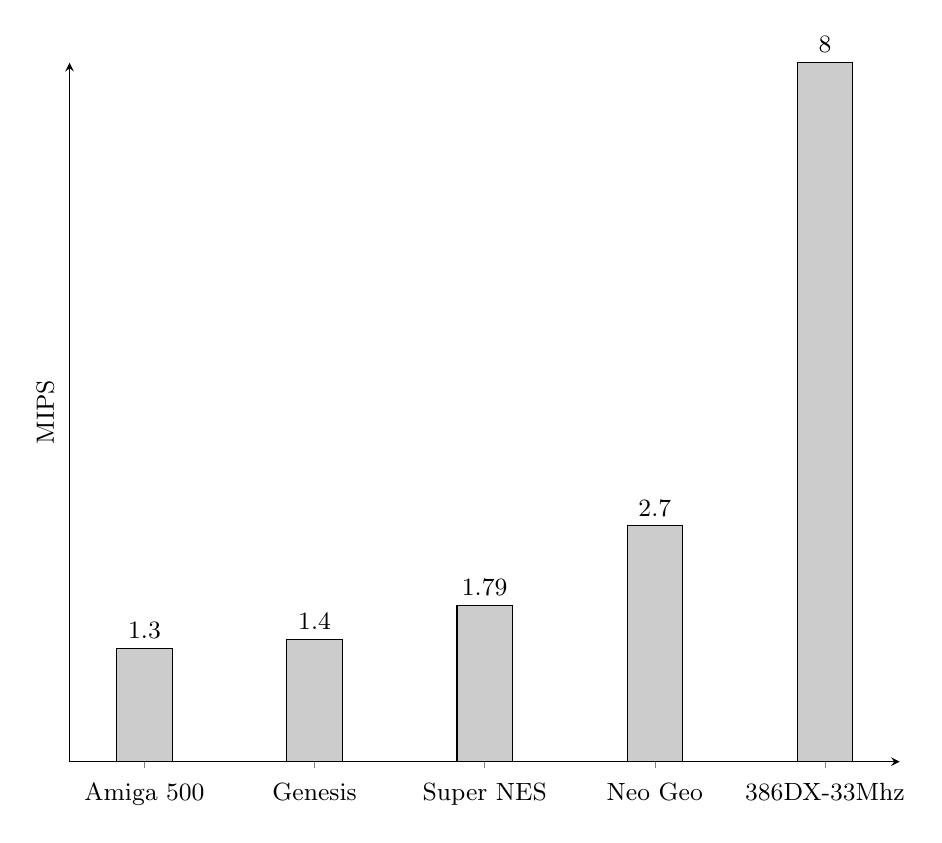
\begin{tikzpicture}[font=\small]
    \begin{axis}[
      width=\textwidth,
      %height=0.6\textwidth,
      ybar=6pt,
      bar width=20pt,
      ylabel={MIPS},
      ymin=0,
      ytick=\empty,
      xtick=data,
      axis x line=bottom,
      axis y line=left,
      enlarge x limits=0.11,
      symbolic x coords={Amiga 500, Genesis, Super NES, Neo Geo,386DX-33Mhz},
      xticklabel style={anchor=base,yshift=-\baselineskip},
      nodes near coords={\pgfmathprintnumber\pgfplotspointmeta}
    ]
      \addplot[fill=black!20,draw=black] coordinates {
        (Amiga 500,1.3)
        (Genesis,1.4)
        (Neo Geo,2.7)
        (Super NES,1.79)
        (386DX-33Mhz,8)
      };
    \end{axis}
   \end{tikzpicture}
   \caption{Consoles\protect\footnotemark Vs PC, CPU comparison with MIPS\protect\footnotemark.}
   \label{fig:ems_xms_layout}
 \end{figure}
 \footnotetext{Million Instructions Per Second.}
 \footnotetext{The Amiga 500, Genesis and Neo-Geo feature a Motorola 68000 CPU respectively running at 7.16 MHz, 7.6 MHz, and 12 Mhz. The Super NES uses a WDC 65816 CPU which is a 8/16 bit version of a 6502 also running at a higher frequency: 3.58 MHz.}
